\section{绪论}
\subsection{选题背景}
随着我国经济社会的快速发展,人们的生活水平显著提高,汽车保有量的持续呈现增长趋势。据中国汽车工业协会数据显示,2023年汽车产销分别完成3016.1万辆和3009.4万辆,同比分别增长11.6\%和12\% ,如图~\ref{fig:cars_sales} 所示。这表明汽车在我国的普及和使用呈现出强劲的发展态势。
\begin{figure}[!htb]
  \centering
  \includesvg[width=0.7\linewidth]{1/汽车销量}
  \caption{\label{fig:cars_sales}2022-2023年中国汽车销量及增长率\\(数据来源:中国汽车工业协会)}
\end{figure}

随着城镇化进程加速\cite{XXCZ202306017},城市密度激增\cite{JZXB201004006},土地资源紧缺问题逐渐凸显。而在这种情况下,人们对于汽车的购买欲望提升,车辆的增加虽然带来了便捷的生活,但也造成了交通系统压力大、停车基础设施不足等问题\cite{CSDQ200708009},如何充分利用停车资源、开发地下停车场\cite{JSSD201905002}并增加经济效益等成为当前城市发展的紧迫问题。

其中,建造地下停车场是一种极为有效的解决方案。同等土地面积下,相较于传统的露天停车场,地下停车场能够提供更多的停车位\cite{1022811825.nh},同时也能节省城市建设用地。此外,地下车库还能有效地缓解地面动静态交通矛盾\cite{CSDQ201807120}。虽然地下车库有诸多优点,但仍存在以下问题:
\begin{enumerate}
  \item 规范不统一。各个公司均用私有规范,导致产生行业壁垒,行业无法快速进步。
  \item 设计参数多。除去政策、法律等规定的固定参数\cite{ZGBZ202119043},还包含了一些不容建筑公司定制化的可变参数。
  \item 结构复杂。相较于地上停车场,地下停车场结构更为复杂。
\end{enumerate}

以上原因,均加剧了地下车库设计远远落后于地上的情况。

在大量建设地下停车场的同时,由于设计师的设计流程较为耗时,未能满足开发商对于周期、质量等的成本要求,因此他们将目光转移到了“一键式”生成设计图。与此同时,Autodesk\cite{carrasco2005innovative,JCJG202304039}等公司开发了一款适用于建筑行业的设计软件AutoCAD,为设计师进行图纸修改提供了更便捷的方式。

基于以上背景,本文致力于设计和开发基于机器学习的车位自动化排布算法并进行可视化展示。
\subsection{选题意义}
\subsubsection{现实意义}
  \paragraph{减轻设计压力} 大幅缩短设计师的设计流程,简化一些较为简单的设计,减少低效的重复劳作。
  \paragraph{提供多种方案} 针对同一初始场地,可利用不同算法进行设计,可能会出现不同的排布方案,便于设计师进行选择。
  \paragraph{降低修改成本} 面对一些特殊情况,如需求改变、车位尺寸改变等,只需付出较少的成本便可重新设计和布局。
\subsubsection{技术意义}
  \paragraph{跨学科融合} 通过将一个较为复杂的地库设计问题转化为计算机可以解决的问题,探究如何将计算机和建筑学进行有机融合,推动计算机辅助设计的进一步发展。

\subsection{非技术因素分析}
非技术因素直接关系到解决方案的实际应用和社会影响。针对本项目提出的基于智能体行为导向和PER-D3QN的车位排布算法,需考虑以下的非技术因素:
\begin{enumerate}
  \item 社会效益: 本项目有望为城市交通管理和城市规划带来积极的影响。通过提高地库设计效率和灵活性,可以更好地满足城市居民和企业的停车需求,缓解城市交通拥堵问题,提升城市交通运行效率,提高城市生活质量。
  \item 经济效益: 地库的建设和管理是一项巨大的经济投资,因此,提高设计效率和降低设计成本对于开发商和设计方都具有重要意义。这项解决方案有望降低地库建设的成本,并提高停车场的利用率,从而提升经济效益。
   \item 环境影响: 地库的建设可能会对周边环境产生一定的影响,如土地利用、地下水位、地质结构等方面。因此,在设计和建设过程中需要充分考虑环境保护和生态平衡,采取相应的环境保护措施,减少对周边环境的影响。
  \item 法律风险: 地库的设计和建设涉及到一系列法律法规和政策规定,包括城市规划、建筑设计、土地利用等方面的法律法规。因此,解决方案的实施需要充分遵守相关法律法规,避免可能存在的法律风险和纠纷。
  \item 社会风险: 地库的设计和建设可能会对周边社区和居民生活产生一定的影响,如噪音、振动、施工期间交通阻塞等。因此,在项目实施过程中需要充分考虑社会影响,采取有效的沟通和协调措施,减少社会风险和负面影响。
\end{enumerate}
  
综上所述,解决方案的实施需要综合考虑各种非技术因素,确保能够最大程度地实现社会、经济和环境效益,同时尽量减少法律和社会风险。
\subsection{国内外研究现状与分析}
\subsubsection{国内外研究现状}
1981年时,Fowler\cite{fowler1981optimal}等人证明无约束的平面布局优化问题是NP完全问题,而将地下车位排布可被看作是带空洞的不规则边界布局优化问题。

针对类似矩阵的地下车库,Birgin\cite{birgin2006method, birgin2006orthogonal}等人提出了通过获取哨兵集,利用非线性规划,实现凸区域内的非重叠打包,并在2010年进一步改进\cite{birgin2010orthogonal},使得矩阵可自由旋转。Cassioli\cite{cassioli2010heuristic}等人结合扰动运动和连续扰动,解决凸区域内等矩形填充问题。L{\'o}pez \cite{lopez2018packing}等人提出利用混合整数非线性规划模型解决圆形容器中的排布问题。

而不同于排布,停车位的设计中还需考虑道路相关信息,例如连通性等。Young、Mendat\cite{young1988review, mendat2003perceptions}等人提出了各种影响停车场需求高效设计的指标。而对于车位排布问题也有着一定的研究,Abdelfatah\cite{abdelfatah2014parking}等人利用整数线性规划(ILP)确定最佳停车角度,并适用于不同环境。Syahrini\cite{syahrini2018mathematical}等人应用整数线性规划优化等腰和等边三角形停车场模型。Hasbiyati\cite{hasbiyati2019parking}等人提出了一种平行四边形形式的停车场的排布,其中平行四边形看作为两个三角形的组合来进行计算。Stephan\cite{stephan2021layout}等人探讨了不同分辨率的正交停车混合整数程序与计算量权衡。

有部分研究进一步考虑停车场的障碍、道路、出入口等因素,并将障碍群成为空洞。Huang\cite{huang2020general}等人研究了基于贪婪算法的单双边停车通道布局选择。利润\cite{1021546706.nh}利用网格分割与满足全局约束的贪婪分割应用于多个排布场景。Guo\cite{guo2022optimal}等人利用非线性规划和模糊评判,解决多形状、多入口、多角度车位的停车场问题。

随着机器学习算法的普及,专家逐渐将排布与机器学习算法结合。Xu\cite{xu2007particle}提出了基于粒子群的算法优化圆形容器内矩形物体布局,并在2010年\cite{xu2010genetic}进一步引入有序定位技术和遗传算法均优化了性能。Cassioli\cite{cassioli2010heuristic}提出启发式方法,通过迭代局部搜索和扰动移动解决矩形填充问题。Zhao\cite{zhao2014human}引入人机协作免疫算法,结合PSO和IA解决布局设计问题。马莹\cite{JSGG201820015}等人提出了自适应量子遗传算法,旨在优化问题求解,并提高材料利用率。Nourinejad\cite{nourinejad2018designing}等人,基于排队路构建了混合整数模型,设计了一种启发式算法,利用Benders进行分解。Chen\cite{chen2022arrangement}等人利用遗传算法优化地下车库标准与非标准停车位布局。

同时,随着自动停车或是自动驾驶车辆的出现,车库也将迎来新的革新。Ferreira\cite{ferreira2014self}等人利用车辆自组织网络和自动技术,优化停车场空间和车辆行驶距离。Timpner\cite{timpner2015k}等人提出自动代客泊车优化模型,显著提高停车密度,减少取车时间,Banzhaf\cite{banzhaf2017high}等人基于前面的优化提出了混合整数规划模型。Kong\cite{kong2018capacity}等人开发混合整数非线性模型,量化自动驾驶对停车效率的影响。Siddique\cite{siddique2021puzzle}等人采用基于谜题和最大密度的设计的方法,求解小型停车场的最佳排布结果,并利用用启发式算法求解大型停车场的排布方式。郑聪\cite{TMJZ202104021}等人基于Dynamo可视化编程,通过模拟设计思路进行自动排布车位。

现仍存在大部分的车库轮廓并非规则,且通常有不规则障碍排布,同时,自动驾驶车辆未普及等问题,专家逐渐转向增加更多的限制条件。徐涵喆\cite{1020726891.nh}通过将图纸分为内圈和外圈,并分别使用遗传算法和贪婪算法进行排布,提高了车库的利用率。黄逸彬等人\cite{BJYD202004002}构建了一种基于图形分割方法的混合整数线性规划模型。冯嘉宇\cite{1022674189.nh}采用像素分割和遗传算法,优化内外圈区域的车位排列。

而随着强化学习的兴起,专家也将注意转移到了基于强化学习的地库排布。余光鑫\cite{1020332216.nh}研究了一种针对规则边缘的基于强化学习的地下停车场生成设计策略,通过边铺设道路,边放置车位的方式,使用简单网络结构和进化策略,但时间开销大,无法对不规则场地进行学习。王潇霆\cite{1022674189.nh}则是改进了强化学习内容,通过每走一步就给予奖励,使得智能体只学习如何铺设道路,但奖励非连续,可解释性较差。

\subsubsection{存在问题及分析}
通过对国内外车位自动化排布已有的研究和参考文献进行分析,发现仍存在如下问题:
\begin{enumerate}
  \item 局限性的奖励机制:现有方法主要依赖固定位置搭配的理论分析来确定具体的奖励值,未充分利用周围所有信息进行计算。  
  \item 过度依赖人工干预:需要对图纸进行区域划分和分别处理,缺乏自动化处理的方法。同时,车位铺设依赖于人工设计,缺乏自动化设计的方法。  
  \item 缺乏实际应用强化学习算法的研究:尽管部分研究借鉴了强化学习的思想,但并未实际运用诸如DQN等强化学习算法进行实践。
  \item 出入口位置的后定问题:现有的研究通常先铺路再放置车位,再设置出入口,但实际情况中,出入口位置需由外界交通决定,且通常位于较为中心的位置,这可能导致设计的实用性不强。
  \end{enumerate}

\subsection{研究目标}
为了缓解停车位供应紧张的问题,本研究的主要目标是在满足建筑规范的条件下,尽可能多地增加车位数量。

\subsection{论文结构安排}
本文共分为六个章节,核心为基于智能体行为导向的车位布局算法、基于PER-D3QN的道路铺设算法、实验例证,具体章节结构安排如图~\ref{fig:chapter_structure}。

第一章主要介绍了地库车位排布自动化的背景及意义,国内外近年来的研究、遇到的问题以及论文结构。

第二章主要介绍了文中涉及的地库排布基础知识和主要应用的技术、算法、模型等。

第三章主要介绍了模型的构建方式,将图纸根据一定精度进行划分,同时介绍了车位铺设的方式。通过道路铺设中智能体的朝向和行为,根据周边的障碍情况,判断车位放置的方向、个数与柱网放置。

第四章主要介绍了基于PER-D3QN的道路铺设算法,将图中信息整合输入到网络中,设定合理奖励,根据总奖励对比同一图不同策略的优越性。

第五章主要介绍了模型中的超参数,与王的研究进行比较并展示不同图纸的绘制情况。

第六章主要归纳了本文的主要工作和成果,指出了研究中的不足,并提出未来研究方向和建议。
\begin{figure}[!htb]
  \centering
  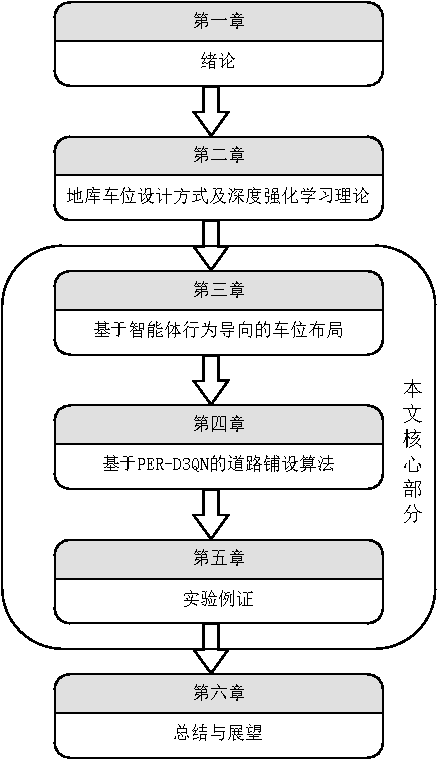
\includegraphics[width=0.75\textwidth]{1/章节结构}
  \caption{论文结构示意图}
  \label{fig:chapter_structure}
\end{figure}